\documentclass[12pt, a4paper]{article}

\usepackage{lastpage}
\usepackage{mathtools}
\usepackage{xltxtra}
\usepackage{libertine}
\usepackage{amsmath}
\usepackage{amsthm}
\usepackage{amsfonts}
\usepackage{amssymb}
\usepackage{enumitem}
\usepackage{xcolor}
\usepackage[left=1.5cm, right=1.5cm, top=2cm, bottom=2cm, bindingoffset=0cm, headheight=15pt]{geometry}
\usepackage{fancyhdr}
\usepackage[russian]{babel}
% \usepackage[utf8]{inputenc}
\usepackage{catchfilebetweentags}
\usepackage{accents}
\usepackage{calc}
\usepackage{etoolbox}
\usepackage{mathrsfs}
\usepackage{wrapfig}

\providetoggle{useproofs}
\settoggle{useproofs}{false}

\pagestyle{fancy}
\lfoot{M3137y2019}
\rhead{\thepage\ из \pageref{LastPage}}

\newcommand{\R}{\mathbb{R}}
\newcommand{\Q}{\mathbb{Q}}
\newcommand{\C}{\mathbb{C}}
\newcommand{\Z}{\mathbb{Z}}
\newcommand{\B}{\mathbb{B}}
\newcommand{\N}{\mathbb{N}}

\newcommand{\const}{\text{const}}

\newcommand{\teormin}{\textcolor{red}{!}\ }

\DeclareMathOperator*{\xor}{\oplus}
\DeclareMathOperator*{\equ}{\sim}
\DeclareMathOperator{\Ln}{\text{Ln}}
\DeclareMathOperator{\sign}{\text{sign}}
\DeclareMathOperator{\Sym}{\text{Sym}}
\DeclareMathOperator{\Asym}{\text{Asym}}
% \DeclareMathOperator{\sh}{\text{sh}}
% \DeclareMathOperator{\tg}{\text{tg}}
% \DeclareMathOperator{\arctg}{\text{arctg}}
% \DeclareMathOperator{\ch}{\text{ch}}

\DeclarePairedDelimiter{\ceil}{\lceil}{\rceil}
\DeclarePairedDelimiter{\abs}{\left\lvert}{\right\rvert}

\setmainfont{Linux Libertine}

\theoremstyle{plain}
\newtheorem{axiom}{Аксиома}
\newtheorem{lemma}{Лемма}

\theoremstyle{remark}
\newtheorem*{remark}{Примечание}
\newtheorem*{exercise}{Упражнение}
\newtheorem*{consequence}{Следствие}
\newtheorem*{example}{Пример}
\newtheorem*{observation}{Наблюдение}

\theoremstyle{definition}
\newtheorem{theorem}{Теорема}
\newtheorem*{definition}{Определение}
\newtheorem*{obozn}{Обозначение}

\setlength{\parindent}{0pt}

\newcommand{\dbltilde}[1]{\accentset{\approx}{#1}}
\newcommand{\intt}{\int\!}

% magical thing that fixes paragraphs
\makeatletter
\patchcmd{\CatchFBT@Fin@l}{\endlinechar\m@ne}{}
  {}{\typeout{Unsuccessful patch!}}
\makeatother

\newcommand{\get}[2]{
    \ExecuteMetaData[#1]{#2}
}

\newcommand{\getproof}[2]{
    \iftoggle{useproofs}{\ExecuteMetaData[#1]{#2proof}}{}
}

\newcommand{\getwithproof}[2]{
    \get{#1}{#2}
    \getproof{#1}{#2}
}

\newcommand{\import}[3]{
    \subsection{#1}
    \getwithproof{#2}{#3}
}

\newcommand{\given}[1]{
    Дано выше. (\ref{#1}, стр. \pageref{#1})
}

\renewcommand{\ker}{\text{Ker }}
\newcommand{\im}{\text{Im }}
\newcommand{\grad}{\text{grad}}

\lhead{Конспект по матанализу}
\cfoot{}
\rfoot{Лекция 6}

\usepackage[]{graphics}

\begin{document}

\section*{Интегральные суммы}

\begin{definition}
    %<*дроблениеотрезка>
    \textbf{Дробление} отрезка $[a,b]$ это разбиение отрезка на $n$ частей следующим образом:
    $$x_0=a<x_1<x_2<\ldots<x_n=b \quad [x_{i-1}, x_i]$$
    %</дроблениеотрезка>
\end{definition}

\begin{definition}
    %<*рангдробления>

    \textbf{Ранг \textit{(мелкость)}} дробления --- длина самого длинного из отрезков дробления:
    $$\tau = \{x_0\ldots x_n\} \quad |\tau|=\max(x_i-x_{i-1})$$
    %</рангдробления>
\end{definition}

\begin{definition}
    %<*оснащение>

    \textbf{Оснащение} --- множество точек $\{\xi_1\ldots \xi_n\} : \xi_i\in[x_{i-1}, x_i]$
    %</оснащение>
\end{definition}

\begin{definition}
    %<*римановасумма>
    \textbf{Интегральная \textit{(риманова)} сумма} для разбиения $\{x_i\}$, произвольной функции $f$ и оснащения $\{\xi_i\}$ это следующая сумма:
    $$\sum_{i=1}^n f(\xi_i)(x_i-x_{i-1})$$
    %</римановасумма>
\end{definition}

%<*римановасуммаграфик>
Геометрически интегральная сумма интерпретируема следующим образом:

\begin{figure}[h]
    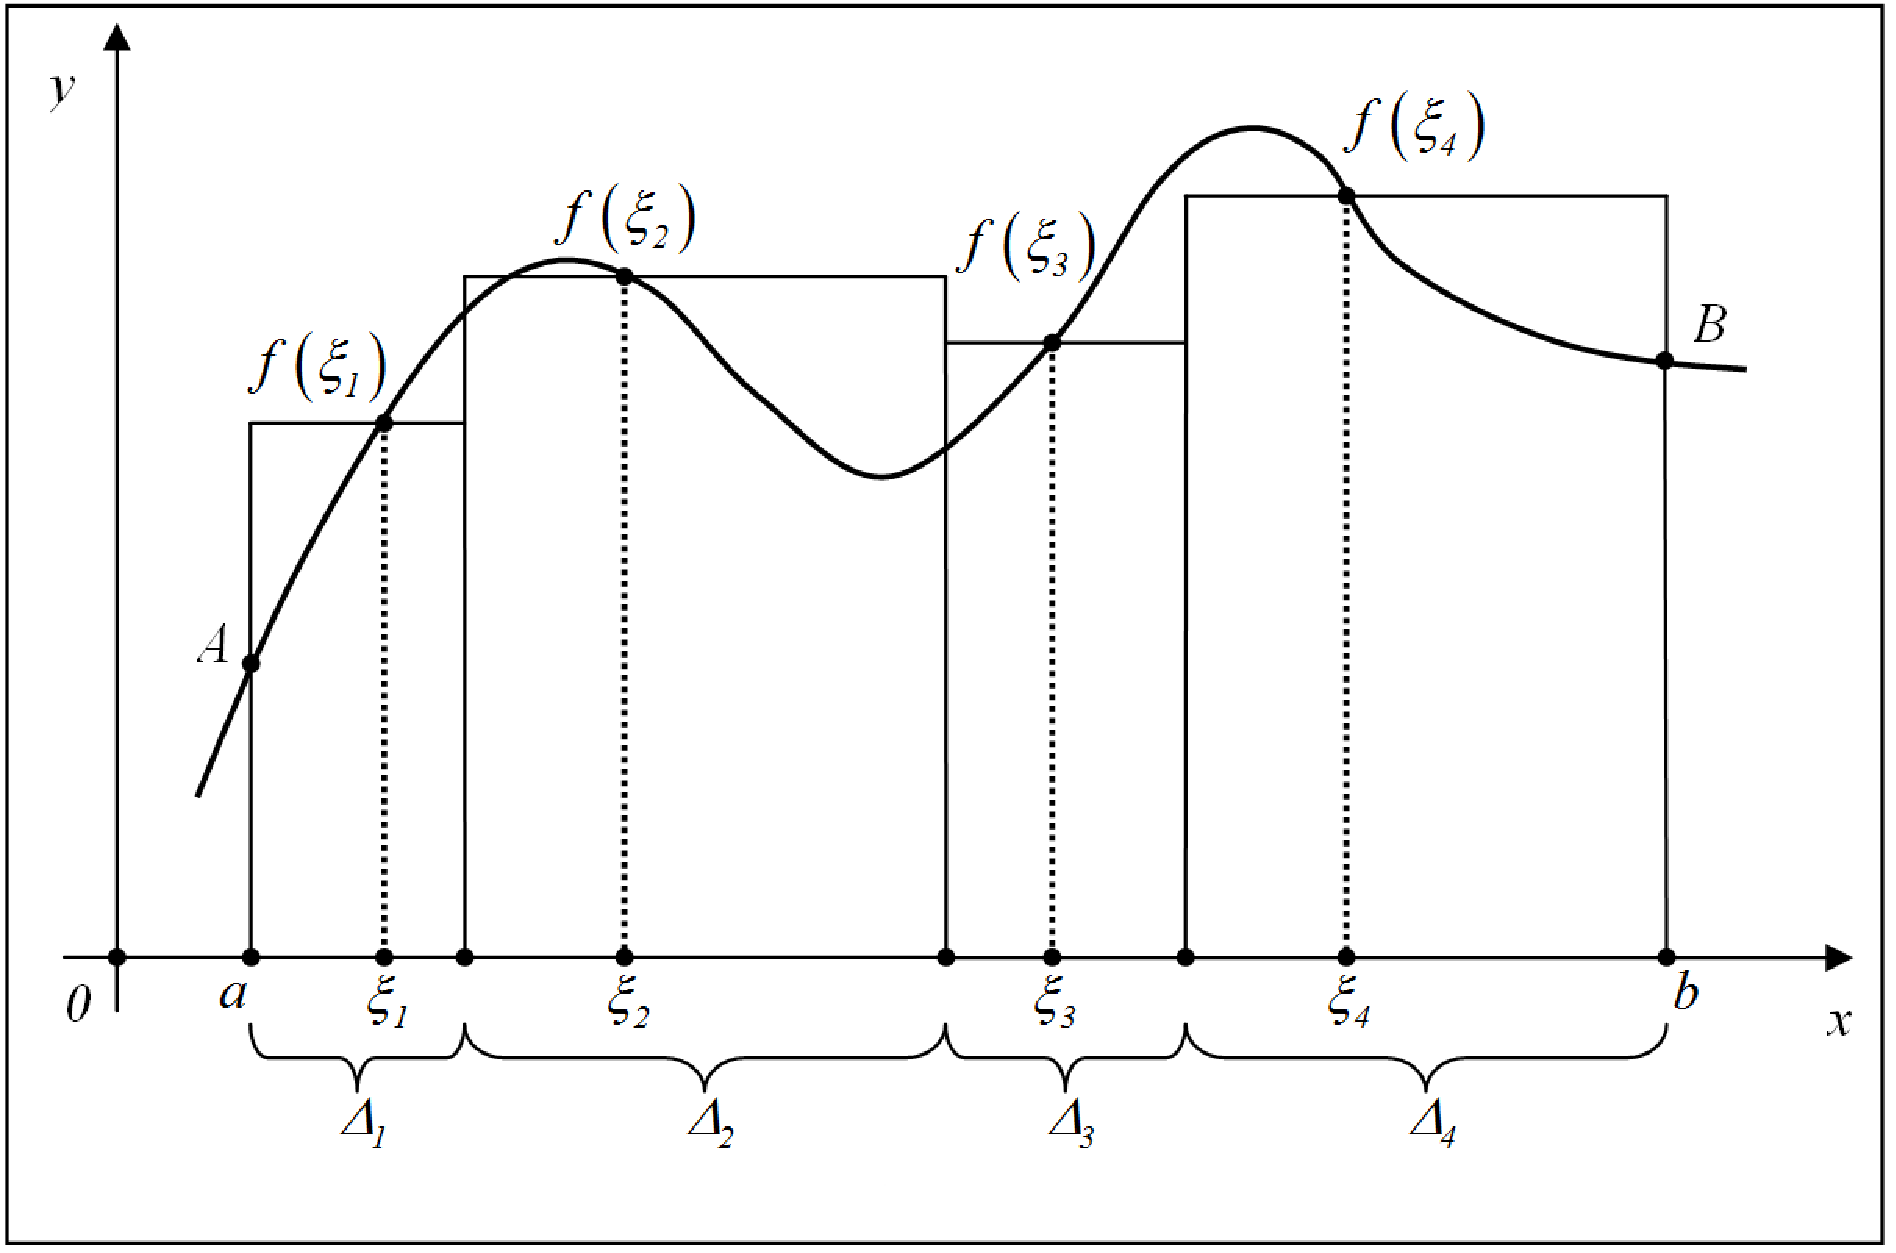
\includegraphics[scale=0.4]{images/riemann-sum.pdf}
    \centering
\end{figure}
%</римановасуммаграфик>

\begin{theorem}
    Об интеграле как пределе интегральных сумм.

    %<*обинтегралекакпределеинтегральныхсумм>
    $f\in C[a,b]$
    $$\forall \varepsilon > 0 \ \ \exists \delta>0 \ \ \forall \text{дробление } \tau=\{x_0\ldots x_n\} : |\tau|<\delta \ \ \forall \text{оснащение } \xi_i:$$
    $$\left|\int_a^b f(x)dx - \sum_{i=1}^n f(\xi_i)(x_i-x_{i-1})\right| < \varepsilon$$
    %</обинтегралекакпределеинтегральныхсумм>
\end{theorem}
%<*обинтегралекакпределеинтегральныхсуммproof>
\begin{proof}
    По теореме Кантора о равномерной непрерывности на компакте.

    $[a,b]$ --- компакт, $f$ непрерывна на $[a,b] \Rightarrow f$ равномерно непрерывна на $[a,b]$:
    $$\forall \varepsilon > 0 \ \ \exists \delta > 0 \ \ \forall x, \overline x\in[a,b] : |x-\overline x|<\delta \quad |f(x)-f(\overline x)|<\varepsilon$$
    По двойной бухгалтерии заменим $\varepsilon$ на $\cfrac{\varepsilon}{b-a}$:
    $$\forall \varepsilon > 0 \ \ \exists \delta > 0 \ \ \forall x, \overline x\in[a,b] : |x-\overline x|<\delta \quad |f(x)-f(\overline x)|<\frac{\varepsilon}{b-a}$$
    Разобьем интеграл на части:
    $$\int_a^b f(x)dx=\sum_{i=1}^n \left(\int_{x_{i-1}}^{x_i} f(x)dx\right)$$
    Запишем $(x_i-x_{i-1})$ в виде интеграла $\int_{x_{i-1}}^{x_i} dx$
    $$\left|\int_a^b f(x)dx - \sum_{i=1}^n f(\xi_i)(x_i-x_{i-1})\right|=\left|\sum_{i=1}^n\left(\int_{x_{i-1}}^{x_i} f(x)dx - f(\xi_i)\int_{x_{i-1}}^{x_i} dx\right)\right|=$$
    $$=\left|\sum_{i=1}^n\int_{x_{i-1}}^{x_i}(f(x)-f(\xi_i))dx\right|\leq\sum\left|\int\right|\leq\sum_{i=1}^n\int_{x_{i-1}}^{x_i}|(f(x)-f(\xi_i))dx|\leq \sum_{i=1}^n\int_{x_{i-1}}^{x_i}\frac{\varepsilon}{b-a}dx=$$
    $$=\frac{\varepsilon}{b-a}\sum_{i=1}^n\int_{x_{i-1}}^{x_i}dx=\frac{\varepsilon}{b-a}\sum_{i=1}^n(x_{i}-x_{i-1})=\frac{\varepsilon}{b-a}(b-a)=\varepsilon$$
\end{proof}
%</обинтегралекакпределеинтегральныхсуммproof>

\begin{remark}
    $f\in C^1[a,b]$; $M:=\max\limits_{x\in[a,b]} |f'(x)|$

    $$|f(x)-f(\overline x)|=|f'(\overline x)(x-\overline x)|\leq M|x-\overline x|$$
\end{remark}

\begin{consequence}
    Равномерное дробление: $x_i=a+\frac{b-a}{n}i; |\tau|=\frac{b-a}{n}$
    $$\int-\sum\leq M(b-a)^2\frac{1}{n}$$
\end{consequence}

\begin{theorem}
    Об интегральных суммах центральных прямоугольников

    %<*обинтегральныхсуммахдляцентральныхпрямоугольников>
    $f\in C^2[a,b] \ \ x_0=a<x_1\ldots <x_n=b \ \ \delta=\max(x_i-x_{i-1}) \ \ \xi_i:=\frac{x_{i-1}+x_i}{2}$. Тогда
    $$\left|\int_a^b f-\sum_{i=1}^n f(\xi_i)(x_i-x_{i-1})\right|\leq \frac{\delta^2}{8}\int_a^b |f''|dx$$
    %</обинтегральныхсуммахдляцентральныхпрямоугольников>
\end{theorem}
%<*обинтегральныхсуммахдляцентральныхпрямоугольниковproof>
\begin{proof}
    $$\int_{x_{i-1}}^{x_i} f(x)dx = \int_{x_{i-1}}^{\xi_i} f(x)dx + \int_{\xi_i}^{x_i} f(x)dx = \int_{x_{i-1}}^{\xi_i} f(x)d(x-x_{i-1}) + \int_{\xi_i}^{x_i} f(x)d(x-x_i)=$$
    $$=f(x)(x-x_{i-1})\Big|_{x=x_{i-1}}^{x=\xi_i}-\int_{x_{i-1}}^{\xi_i} f'(x)(x-x_{i-1})dx+f(x)(x-x_i)\Big|^{x=x_{i}}_{x=\xi_i} - \int_{\xi_i}^{x_i} f'(x)(x-x_{i-1})dx=(*)$$
    Заметим, что $\xi_i-x_{i-1}=x_i-\xi_i$, поэтому $f(x)(x-x_{i-1})\Big|_{x=x_{i-1}}^{x=\xi_i}+f(x)(x-x_i)\Big|^{x=x_{i}}_{x=\xi_i}=f(\xi_i)(x_i-x_{i-1})$
    $$(*)=f(\xi_i)(x_i-x_{i-1}) - \Big( f'(x) \frac{(x-x_{i-1})^2}{2} \Big|_{x_{i-1}}^{\xi_i} - \frac{1}{2} \int_{x_{i-1}}^{\xi_i} f''(x)(x-x_{i-1})^2 dx +$$
    $$+f'(x)\frac{(x-x_i)^2}{2} \Big|^{x_i}_{\xi_i} - \frac{1}{2} \int_{\xi_i}^{x_i} f''(x)(x-x_i)^2 dx \Big)=$$
    $$=f(\xi_i)(x_i-x_{i-1})-0+\frac{1}{2}\int_{x_{i-1}}^{x_i} f''(x)\varphi(x)dx$$
    $$\varphi(x)= \begin{cases}
        (x-x_{i-1})^2, & x\in [x_{i-1}, \xi_i] \\
        (x-x_i)^2, & x\in [\xi_i, x_i]
    \end{cases}$$
    Итого:
    $$\int_a^b f(x)=\sum_{i=1}^n f(\xi_i)(x_i-x_{i-1})+\frac{1}{2}\int_a^b f''(x)\varphi(x)dx$$
    $$\left| \int - \sum \right| \leq \frac{1}{2}\int_a^b |f''(x)|\varphi(x)dx$$
    $$\max_{x\in[a,b]}\varphi(x)\stackrel{\text{достигается на отрезке длины }\delta}{=}\frac{\delta^2}{4}$$
    $$\frac{1}{2}\int_a^b |f''(x)|\varphi(x)dx\leq\frac{\delta^2}{8}\int_a^b |f''|$$
\end{proof}
%</обинтегральныхсуммахдляцентральныхпрямоугольниковproof>

\begin{theorem}
    О формуле трапеций. 

    %<*теоремаоформулетрапеций>
    $f\in C^2[a,b], \tau, \delta=|\tau|$

    Тогда
    $$\left|\int_a^b fdx - \sum \frac{f(x_i) + f(x_{i-1})}{2} (x_i-x_{i-1}) \right|\leq\frac{\delta^2}{8}\int_a^b |f''|$$
    %</теоремаоформулетрапеций>
\end{theorem}
%<*теоремаоформулетрапецийproof>
\begin{proof}
    Берем $\xi_i=\frac{x_{i-1}+x_i}{2}$
    $$\int_{x_{i-1}}^{x_i} f(x)dx=\int_{x_{i-1}}^{x_i} f(x)d(x-\xi_i)=f(x)(x-\xi_i)\Bigg|_{x_{i-1}}^{x_i} - \int_{x_{i-1}}^{x_i}f'(x)(x-\xi_i)dx=$$
    $$=(f(x_i)+f(x_{i-1}))\frac{x_i-x_{i-1}}{2} - \int_{x_{i-1}}^{x_i}f'(x)\cdot \left(-\frac{1}{2}\right)d((x-x_{i-1})(x_i-x))=(*)$$
    Проверим, что замена выражения под дифференциалом верная:
    $$((x-x_{i-1})(x_i-x))'=(-x^2+x(x_i+x_{i-1})-x_{i-1}x)'=-2\left(x-\frac{x_i+x_{i-1}}{2}\right)$$
    Действительно верно.
    $$\psi(x):=(x-x_{i-1})(x_i-x)$$
    $$(*)=(f(x_i)+f(x_{i-1}))\frac{x_i-x_{i-1}}{2} + \frac{1}{2}f'(x)(x-x_{i-1})(x_i-x)\Bigg|_{x_{i-1}}^{x_i} - \frac{1}{2}\int_{x_{i-1}}^{x_i} f''\psi(x)dx$$
    $$\left| \int - \sum \right|\leq\frac{1}{2}\int_a^b |f''|\psi(x)dx$$
    $$\max \psi = \frac{\delta^2}{4}$$
\end{proof}
%</теоремаоформулетрапецийproof>

\begin{remark}
    $f$ --- выпуклая $( f'' \geq 0 )$

    Тогда $\int - \sum_{\text{пр}} \geq 0$, $\int - \sum_{\text{тр}} \leq 0$
\end{remark}

\begin{example}
    $$\lim_{n\to+\infty} \sum_{k=1}^n \frac{k}{k^2+n^2+1}=?$$
    $[a, b] := [0, 1], x_i=\frac{i}{n}, \xi_k=\frac{k}{n}$ (дробление равномерное)


    $$\lim_{n\to+\infty} \sum_{k=1}^n \frac{k}{k^2+n^2+1} = \lim_{n\to+\infty} \sum_{k=1}^n \frac{\frac{k}{n}}{\left(\frac{k}{n}\right)^2 + 1 + \frac{1}{n^2}} \frac{1}{n} \stackrel{\text{по рукомаханию}}{\approx} \lim_{n\to+\infty} \sum_{k=1}^n \frac{\frac{k}{n}}{\left(\frac{k}{n}\right)^2 + 1} \frac{1}{n}=$$
    По теореме
    $\sum f\left(\xi_k\right)\frac{1}{n}=\sum f\left(\frac{k}{n}\right)\frac{1}{n}\xrightarrow{n\to\infty}\int_0^1 f(x)dx$
    $$=\int_0^1 \frac{x}{x^2+1}dx = \frac{1}{2}\ln(x^2+1)\Bigg|_0^1 = \frac{1}{2}\ln 2$$
    Вернемся к рукомаханию. Мы заменили $\frac{1}{n^2}$ на $0$ \textit{(эквивалентную)} при $n\to\infty$, тем самым совершив ``небольшую ошибку''. Но эта ошибка совершена в $n$ слагаемых, т.е. у нас много небольших ошибок, а это может быть большой ошибкой. Докажем, что разность выражения с заменой и выражения без замены бесконечно мала:
    $$\left|\sum_{k=1}^n \frac{\frac{k}{n}}{\left(\frac{k}{n}\right)^2 + 1 + \frac{1}{n^2}} - \sum_{k=1}^n \frac{\frac{k}{n}}{\left(\frac{k}{n}\right)^2 + 1}\right| \leq \sum_{k=1}^n \left|\frac{1}{n}\frac{k}{n}\frac{-\frac{1}{n^2}}{(\left(\frac{k}{n}\right)^2 + 1 + \frac{1}{n^2})(\left(\frac{k}{n}\right)^2 + 1)}\right|\leq$$
    $$\leq\sum\frac{1}{n^3}1 \frac{1}{1\cdot 1}=\frac{1}{n^2}\xrightarrow{n\to+\infty}0$$
\end{example}

Простейший случай формулы Эйлера-Маклорена

%<*формулаэйлерамаклорена>
$m, n\in \Z, f\in C^2[m, n]$. Тогда
$$\int_m^n f(x)dx=\left(\sum_{i=m}^n\right)' f(i)-\frac{1}{2}\int f ''(x)\{x\}(1-\{x\})dx$$
$'$ означает, что крайние слагаемые берутся с весом $\frac{1}{2}$, $\{x\}$ --- дробная часть $x$
%</формулаэйлерамаклорена>

%<*формулаэйлерамаклоренаproof>
\begin{proof}
    Это очевидно по формуле трапеций: $x_i:=i$
    $$\int_m^n f(x)dx = \sum_{i=m+1}^n \frac{f(i)+f(i-1)}{2}\cdot 1 - \frac{1}{2}\int_m^n f''(x) \psi(x)$$
    $$\psi(x)\stackrel{def}{=}(x-x_{i-1})(x_i-x)=(x-i+1)(i-x)=(x-i+1)(1-(x-i+1))=\{x\}(1-\{x\})$$

    $f(n)/2$ и $f(m)/2$ в сумму попадают только 1 раз, остальные --- 2 раза, как и в искомой формуле.
\end{proof}
%</формулаэйлерамаклоренаproof>

Обычно эта формула используется, чтобы из суммы получить интеграл, а не наоборот.

\begin{example}
    %<*асимптотикастепенныхсумм>
    $p > -1 \quad f(x)=x^p$
    $$1^p+2^p+\ldots n^p=\int_1^n x^p dx + \frac{1}{2} 1^p+\frac{1}{2}n^p+\frac{1}{2}\int_1^n p(p-1) x^{p-2}\{x\}(1-\{x\})=$$
    $\frac{1}{2} 1^p+\frac{1}{2}n^p$ добавлены, чтобы не писать слева деление крайних слагаемых на 2.
    $$=\frac{n^{p+1}}{p+1} - \frac{1}{p+1}+\frac{1}{2}+\frac{1}{2}n^p+\mathcal O(\max(1, n^{p-1}))=(*)$$
    Откуда появилось $\mathcal O$? $\{x\}(1-\{x\})<1 \Rightarrow \int_1^n p(p-1) x^{p-2}\{x\}(1-\{x\})\leq C(n^{p-1}-1)$, $C$ --- некоторая константа.

    Занесем константы под $\mathcal O$:
    $$(*)=\frac{n^{p+1}}{p+1} + \frac{1}{2}n^p + \mathcal O(\max(1, n^{p-1}))$$
    %</асимптотикастепенныхсумм>

    $$] p = -\frac{1}{2} \quad 1+\frac{1}{\sqrt 2} + \frac{1}{\sqrt 3} + \ldots + \frac{1}{\sqrt n} = 2\sqrt n + \mathcal O(1)$$
    $$] p = \pi \quad 1^\pi + 2^\pi + \ldots + n^\pi = \frac{n^{\pi + 1}}{\pi + 1} + \frac{1}{2}n^\pi + \mathcal O(n^{\pi - 1})$$
    $$] p = 1 \quad 1 + 2 + \ldots + n = \frac{n^2}{2} + \frac{n}{2} + \mathcal O(1)=\frac{n^2}{2}+\frac{n}{2}$$
    $\mathcal O(1)=0$ в данной ситуации, т.к. при интеграле $p-1=0$ и $\frac{1}{2}$ сократилось с подстановкой в первый интеграл 1.
    %<*асимптотикачастичныхсуммгармоническогоряда>
    $$] p = -1 \quad 1+\frac{1}{2}+\ldots+\frac{1}{n}=\ln n+\frac{1}{2}+\frac{1}{2n} + \int_1^n x^{-3}\{x\}(1-\{x\})=(*)$$
    $$\int_1^n x^{-3}\{x\}(1-\{x\}) \leq \frac{1}{4}\int_1^n \frac{dx}{x^3} = \frac{1}{8}\frac{-1}{\alpha^2}\Bigg|_1^n=\frac{1}{8}\left(1-\frac{1}{n^2}\right)<\frac{1}{8}$$
    $$(*)=\ln n + \gamma + o(1) \quad \gamma\in\left[\frac{1}{2}, \frac{1}{2}+\frac{1}{8}\right]$$
    %</асимптотикачастичныхсуммгармоническогоряда>
    \begin{definition}
        %<*постояннаяэйлера>
        $\gamma$ --- \textbf{постоянная Эйлера}. $\approx 0.577$
        $$\gamma = \lim_{n\to\infty}\left(\sum_{k=1}^n\frac{1}{k} - \ln n\right)$$
        %</постояннаяэйлера>
    \end{definition}
    %<*формуластирлингаproof>
    $$] f(x) = \ln x \quad \ln 1 + \ln 2 + \ldots + \ln n = \int_1^n \ln x dx + \frac{\ln n}{2} - \frac{1}{2} \int_1^n \frac{\{x\}(1-\{x\})}{x^2}dx=$$
    $$= n\ln n - n + 1 + \frac{\ln n}{2} - \frac{1}{2}\frac{1}{4}\int_1^n \frac{1}{x^2} + o(1) = n\ln n - n + \frac{\ln n}{2} + C_1 + o(1)$$
    $$\ln 1 + \ln 2 + \ldots + \ln n = \ln n!$$
    $$n! = e^{n\ln n - n + \frac{\ln n}{2} + C_1 + o(1)}$$
    $$n! = n^n e^{-n} \sqrt n e^{C_1 + o(1)}\equ_{n\to+\infty} Cn^n e^{-n}\sqrt n$$
    Найдём $C$.
    %</формуластирлингаproof>
\end{example}

\subsection*{Формула Валлиса}

%<*формулаваллисаproof>

Вывод формулы Валлиса:
$$I_n := \int_0^{\frac{\pi}{2}} \sin^n x dx = \left[\begin{array}{rl}
    u = \sin^{n-1} x & du = (n-1)\sin^{n-2} x \cos x dx \\
    dv = \sin x dx & v = -\cos x
\end{array}\right]=$$
$$=-\cos x \sin^{n-1} x \bigg|_0^{\frac{\pi}{2}} + \int_0^{\frac{\pi}{2}} \cos^2 x (n-1)\sin^{n-2} x dx=$$
$$(n-1) \int_0^{\frac{\pi}{2}} (1-sin^2 x) \sin^{n-2} x =(n-1) (I_{n-2}-I_n)$$
$$I_n=\frac{n-1}{n}I_{n-2}=\frac{n-1}{n}\frac{n-3}{n-2}I_{n-4}=\frac{n-1}{n}\frac{n-3}{n-2}\frac{n-5}{n-4}I_{n-6}=\ldots=\begin{cases}
    \frac{(n-1)!!}{n!!} \frac{\pi}{2} , & n \text{ --- чёт.} \\
    \frac{(n-1)!!}{n!!}1 , & n \text{ --- нечет.}
\end{cases}$$

$$\sin^{2k+1} x \leq \sin^{2k} x \leq \sin^{2k-1} x$$
Проинтегрируем по $\left[0, \frac{\pi}{2}\right]$:
$$\frac{(2k)!!}{(2k+1)!!} \leq \frac{(2k-1)!!}{(2k)!!}\frac{\pi}{2} \leq \frac{(2k-2)!!}{(2k-1)!!}$$
$$\left(\frac{(2k)!!}{(2k-1)!!}\right)^2 \frac{1}{2k+1} \leq \frac{\pi}{2} \leq \left(\frac{(2k)!!}{(2k-1)!!}\right)^2 \frac{1}{2k}$$
$$\text{Правая часть $-$ левая часть} = \left(\frac{(2k)!!}{(2k-1)!!}\right)^2\left(\frac{1}{2k}-\frac{1}{2k+1}\right)=\left(\frac{(2k)!!}{(2k-1)!!}\right)^2\frac{1}{2k}\frac{1}{2k+1}\leq \frac{\pi}{2}\frac{1}{2k}\xrightarrow{k\to+\infty}0$$
Таким образом, левая и правая части стремятся друг другу и зажимают $\pi/2$.
%</формулаваллисаproof>
%<*формулаваллиса>
$$\lim_{k\to+\infty}\left(\frac{(2k)!!}{(2k-1)!!}\right)^2\frac{1}{2k}=\frac{\pi}{2}$$
%</формулаваллиса>
$$\lim_{k\to+\infty}\frac{(2k)!!}{(2k-1)!!}\frac{1}{\sqrt k}=\sqrt \pi$$

Вернемся к нахождению $C$.
%<*формуластирлингаproof2>
$$\sqrt \pi =  \lim_{k\to+\infty}\frac{2\cdot4\cdots(2k)}{1\cdot3\cdots(2k-1)}\frac{1}{\sqrt k}=$$
Домножим дробь на числитель:
$$=\lim_{k\to+\infty} \frac{1}{\sqrt k}\frac{2^2\cdot4^2\cdots(2k)^2}{(2k)!}=$$
Вынесем $2$ из каждого множителя в числителе:
$$=\lim_{k\to+\infty} \frac{1}{\sqrt k}\frac{(2^k k!)^2}{(2k)!}=$$
Замена на эквивалент:
$$=\lim_{k\to+\infty} \frac{1}{\sqrt k}\frac{(2^k Ck^k e^{-k}\sqrt k)^2}{C (2k)^{2k} e^{-2k}\sqrt{2k}}=\lim_{k\to+\infty} \frac{C}{\sqrt 2}=\frac{C}{\sqrt 2}$$
$$C=\sqrt{2\pi}$$
%</формуластирлингаproof2>
%<*формуластирлинга>
$$n! \equ_{n\to+\infty} n^n e^{-n}\sqrt n\sqrt {2\pi}$$
%</формуластирлинга>
Это формула Стирлинга.
\end{document}